\icode{E-MV-SI-L1-260627-001}
一列沿\(x\)轴正方向传播的简谐机械横波，波速为\,\qty{4}{m/s}。某时刻波形如图所示，下列说法正确的是\paren[D]

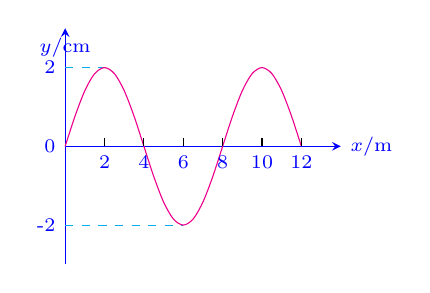
\begin{tikzpicture}[>=stealth,font=\scriptsize]
    \draw[->,blue] (0,0)node[left]{0}--(3.5,0)node[right]{\(x\)/\qty{}{m}};
    \draw[->,blue] (0,-1.5)--(0,1.5)node[below]{\(y\)/\qty{}{cm}};
    \draw[dashed,cyan] (0,1)node[left,blue]{2}--(.5,1) (0,-1)node[left,blue]{-2}--(1.5,-1);
    \draw[domain=0:3,smooth,magenta] plot(\x,{sin((pi*\x) r)});
    \foreach \x/\n in {.5/2,1/4,1.5/6,2/8,2.5/10,3/12}
      \draw (\x,.1)--(\x,0)node[below,blue]{\(\n\)};
\end{tikzpicture}
\begin{choices}
    \item 这列波的振幅为\qty{4}{cm}
    \item 这列波的周期为\qty{1}{s}
    \item 此时\(x =\) \,\qty{4}{m}处质点沿\(y\)轴负方向运动
    \item 此时\(x =\) \,\qty{4}{m}处质点的加速度为0
\end{choices}
\begin{answer}
    D
\end{answer}